\chapter{Systemvalg}
\label{chap:systemvalg}
%introduktion. formål, metoder -> resultat
Dette kapitel beskriver, hvordan vi er kommet frem til de overordnede egenskaber, som vores system skal have. Dette blev opnået vha. interviews med informanterne. På baggrund af interviewene, udformede vi systemdefinitioner, som definerede systemer der havde til formål at mindske madspild. Til sidst vælges endelig systemdefinition, der stemmer overens med informanternes behov og BATOFF-kriterierne, som er forklaret yderligere i \secref{sec:systemdefinition}.

%Dette kapitel viser, hvordan vi kommer frem til den endelige systemdefintion.


\section{Beskrivelse af situationen}
\label{sec:situation}

%indledning
To familier kan ikke repræsentere en befolknings madvaner eller madlavningspolitik. Vi er helt klare over, at vores to informanters madvaner ikke kan generaliseres til hele Danmark. Vi vurderer dog, at samtalerne med informanterne giver et godt billede af, hvordan stituationen, mht. madlavningen og madvaner, ser ud i nogle danske husstande. Merete og Keld kommer fra to forskellige familier i Aalborg.

%situation
Situation er, at begge vore informanter står for madlavningen i deres husstande. De er begge opmærksomme på, at der er dele af aftensmaden, der bliver smidt ud. Denne madspild forekommer selvom, de prøver at genbruge madresterne ved bl.a. at fryse madresterne ned eller genbruge dem den kommende dag i \fx biksemad, supper osv. Det forekommer ofte, at familierne får gårsdagens rester til dagens aftensmad.

%madvaner og madlavning
Det er vigtigt at være opmærksom på, at Merete har været vant til at lave aftensmad til to drenge og en pige ud over hende selv og hendes mand. Ægteparrets børn er flyttet hjemmefra, og de spiser derfor sjældent med hos forældrene. Det er svært at få mængden af aftensmad til at passe, så der ikke er nogen rester, når alle er mætte. Merete er også meget opmærksom på holdbarhedsdatoerne på de forskellige madvarer. Hvis den dato bliver overskredet, så bliver maden smidt ud med det samme.

Derudover forklarer Keld, at han med vilje laver ekstra store portioner til aftensmaden, så familien kan få resterne fra dagens aftensmad den næste dag. Denne strategi benytter Keld sig af, fordi han mener, at der ikke altid er meget tid tilovers til madlavningen. Ægteparret har to små børn, der skal passes og bruges tid på. Ud over at tage sig af børnene, så har de også hver deres arbejde, som skal ses til. Derfor er tid ikke noget, som ægteparret har meget af, og de bruger lignende tricks til at bruge mindre tid på madlavningen og mere tid på at være sammen. Det er helt tydeligt, at tiden er en vigtig faktor for Kelds familie, og det er netop derfor, at familien ofte får de samme retter til aftensmad.

%indkøbsliste
Når det kommer til indkøb af madvarer, så er det ikke altid, at der bliver brugt en indkøbsseddel til at planlægge indkøbet. Den person, der har tid, handler ind. Merete og hendes mand kan bedst lide at gå på opdagelse i supermarkedet, og se om de kan finde nogle gode tilbud, som de kan lave noget aftensmad ud af. Keld derimod står altid for indkøb, og han har ofte en plan i hovedet eller en liste i hånden over, hvad han skal have købt med hjem til aftensmaden. Han påpeger, at det ofte forekommer, at han får købt lidt andet godt (slik osv.) med hjem end der stod på indkøbssedlen.

%madplan
Hverken Merete eller Keld benytter sig af en madplan, når ugens aftensmad skal planlægges. De har ofte idéerne til aftensmaden i hovedet, og madlavningen er rutinepræget. Aftensmaden er meget ensformig, fordi fremgangsmåden er velkendt og derved nem og hurtig at lave. Derudover er det svært for familierne at planlægge tidspunktet for aftensmaden, fordi de alle har jobs, der skal ses til. Derfor ændrer deres planer sig pludseligt, og det vil være svært at styre en madplan, når arbejdstiderne kan variere.

\begin{figure}
\centering
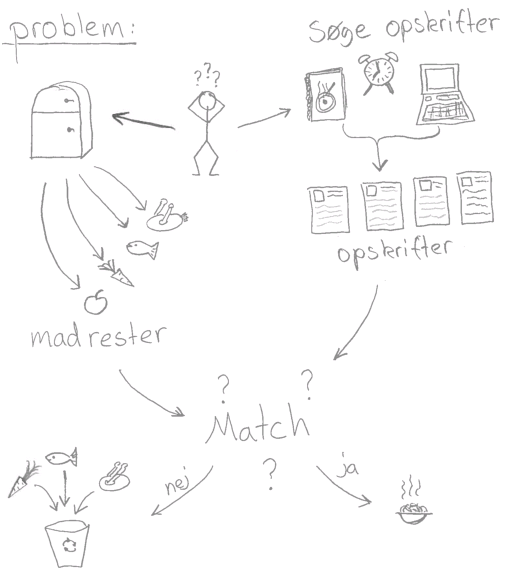
\includegraphics[scale=0.6]{billeder/rigebilleder/problemomraade.png}
\capt{Rigt billede, der visualiserer problemet ved at skulle genbruge madrester.}
\label{fig:rigbillede1}
\end{figure}

Det rige billede i \figref{fig:rigbillede1} viser en bruger, der ikke har tid eller ressourcer til at finde ud af, hvordan madresterne, der er i køleskabet, kan blive brugt i madlavningen. Det rige billede har hjulpet os til at få en forståelse for situationen.

%afslutning
På baggrund af samtalerne med informanterne, skal vi udarbejde systemdefinitioner og udvælge en af disse, som vi skal basere vores videre arbejde på. For at være i stand til at udarbejde systemdefinitioner effektivt, har vi valgt at undersøge nogle eksisterende systemer, der forsøger at løse en lignende problemstilling, som den vi arbejder med.
\section{Eksisterende systemer}
\label{sec:eksisterendesystemer}

På baggrund af samtalerne med informanterne, har vi udarbejded systemdefinitioner og udvalgt en af disse, som vi har basered vores videre arbejde på. For at være i stand til at udarbejde systemdefinitioner effektivt, valgte vi at undersøge nogle eksisterende systemer, der forsøger at løse en lignende problemstilling, som den vi arbejdede med.

Der eksisterer allerede en lang række systemer, som tilbyder en service, der ligner den, som vi ønsker at kunne tilbyde. Heriblandt valgte vi at undersøge  eksisterende danske systemer, nemlig Forbrugerrådets \href{https://play.google.com/store/apps/details?id=com.nodes.forresten}{For Resten} \cite{forresten}, \href{http://www.dk-kogebogen.dk/}{DK-kogebogen} \cite{dkkogebogen} og \href{http://opskrifter.dk/}{Opskrifter.dk} \cite{opskrifterdk}. Der eksisterer desuden også en række engelske hjemmesider, som vi ikke var interesseret i. Dette er grundet, at de dansksprogede anses som værende direkte konkurrenter til Foodl. For Resten er en mobilapplikation kun tilgængelig på iOS- og Android-smartphones. DK-kogebogen og Opskrifter.dk er webapplikationer tilgængelig på internettet. Efter møde 1 med informanterne blev der diskuteret nogle kriterier, som de synes er vigtige for brugervenligheden og funktionaliteten, der gør opskriftshjemmesider så tiltrækkende som muligt. Vi besluttede os for, at der var nogle egenskaber, der er mere relevante at undersøge end andre. De følgende egenskaber så vi nærmere på i de forskellige systemer:

\begin{itemize}[noitemsep]
  \item Antal opskrifter
  \item Kvalitet af opskrifter
  \item Fleksibilitet
  \item Opskriftssøgningsfunktion
\end{itemize}

Det er relevant at undersøge, hvor mange opskrifter systemerne har i deres databaser. Jo færre opskrifter de har, jo større er risikoen for, at man, som bruger, får nogle tomme resultater, når man søger efter opskrifter med en specifik ingrediens. 

Kvaliteten af opskrifterne er også vigtig. Hvis systemet tillader alle og enhver at uploade deres opskrifter til hjemmesiden, så er der en risiko for at opskrifter vil være fejlfyldt og uden billeder, eller ligefrem ubrugelige hvis der blot mangler \'{e}t trin i fremgangsmåden. Oplever brugeren, gang på gang, fejl i opskrifter eller opskrifter med manglende indhold som søgningsresultater, så vil sidens troværdighed mindskes. 

Hjemmesidens fleksibilitet blev vurderet ud fra om brugeren har mulighed for \fx at op- eller nedskalere opskrifter således, at de er tilpasset flere eller færre personer; om det er muligt at sortere efter tilberedningstid eller andre ting, og om brugeren har mulighed for at sætte begrænsninger op for, hvilke opskrifter han/hun ønsker skal vises (\fx kun opskrifter uden svinekød, laktose, nødder osv.). 

Den sidste funktion, som vi undersøgte, var opskriftssøgningsfunktionen. Her undersøgte vi, hvordan de tre systemer havde valgt at bygge deres tøm-køleskabs-funktion op, \fx hvordan man søger på ingredienser, eller hvor lettilgængelig funktionen er mm.

\subsection{For Resten}
\label{subsec:forresten}

For Resten er en gratis mobilapp, der er udgivet af Forbrugerrådet som en del af en kampagne mod madspild. App’en findes til Android og iOS og kan installeres fra henholdsvis Google Play og App Store. App’en fungerer ved, at man på to ``hjul'' vælger kategori (``Kornprodukter'', ``Mejeriprodukter'', ``Kød og æg'' og fem andre kategorier) og rest (\fx ``Mørbrad'', ``Kylling'', ``Kødsovs'' osv.), hvorefter brugeren præsenteres for en række opskrifter, som inkluderer den valgte rest.

\begin{figure}[H]
\centering
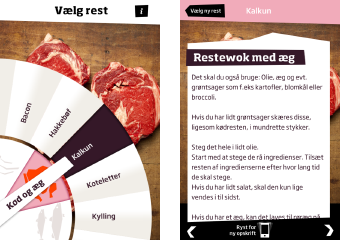
\includegraphics[scale=0.7]{billeder/forbilleder/forresten.png}
\capt{Brugergrænseflade i For Resten. Valg af rest (t.v.) og visning af opskrift (t.h.)}
\label{fig:forresten}
\end{figure}

For hver rest er der ca. 4 - 5 opskrifter, hvilket med 124 rester giver et samlet antal opskrifter på omkring 500 - 600 (dette er vores eget bud på mængden. Det faktiske antal opskrifter er ikke oplyst nogen steder). For opskrifterne vises der kun fremgangsmåde, og ikke en liste over ingredienser. Det er derfor heller ikke muligt at op- eller nedskalere opskrifsportionerne. Derudover er der ingen mulighed for at favorisere opskrifter eller på anden måde gemme resultater af en søgning. I forhold til søgningen så kan man, som sagt, kun søge på én enkelt rest, og ikke sammensætte rester, som ved andre løsninger. Samtidig har man kun mulighed for at vælge sin rest på hjulene, og har altså ikke muligheden for at skrive i et felt. Under afprøvningen var det derfor i nogle tilfælde svært at finde den ønskede ingrediens. Det er de samme problemstillinger, der kommer til udtryk i brugernes anmeldelser af app’en på Google Play. \Fx skriver brugeren \textit{TJA} \cite{tja}:

\begin{quote}
``Fin ide, men den burde være blevet kælet lidt mere for, før den røg i play. Hvem laver restemad af én rest og så en masse ting der skal købes? Jeg har brug for at kunne søge på tre-fire rester for at se, hvordan de kan kombineres til noget spændende. Og hvis jeg finder en opskrift, jeg vil prøve, så kan jeg ikke gemme den i appen, men skal søge den frem igen når jeg står i netto og skal købe de ting, der skal til - og søge den frem igen, når jeg skal lave maden. Alt for besværligt.''
\end{quote}

Sammenlagt har app’en på Google Play bedømmelsen 2,4 stjerner ud af 5, baseret på 69 bedømmelser, hvoraf næsten halvdelen kun har givet app’en 1 stjerne. Et andet kritikpunkt, der kommer til udtryk i flere anmeldelser, er, at app’en bruger for mange systemressourcer og er langsom til at starte op.

\subsection{DK-Kogebogen}
\label{subsec:dk-kogebogen}

DK-Kogebogen er en webapplikation, som tilbyder en lang række funktioner, hvoraf ``Tøm køleskabet'' er en af dem. Udover ``Tøm køleskabet'', tilbyder DK-kogebogen også en ugentlig madplan, en ekstern hjemmeside med fokus på viden omkring mad (energiindhold, vitaminindhold osv.), en kalorieberegner og meget meget mere. Sagt med andre ord, så prioriterer DK-Kogebogen ikke udelukkende sine ressourcer på ``Tøm køleskabet'', og dette kan påvirke kvaliteten af denne. Desuden kan det også være svært at skabe sig et overblik på hjemmesiden, da der er så mange funktioner pakket sammen på samme side. Siden har et omfang af 36.434 opskrifter, hvilket er det klart største antal blandt de undersøgte systemer. De mange opskrifter er indsendt og lavet af brugere af hjemmesiden. Dette kan både være positivt og negativt. Det kan være negativt, da der kan forekomme en del fejl i opskrifterne. DK-Kogebogen skriver på deres hjemmeside, om de indsendte opskrifter:

%kilde: http://www.dk-kogebogen.dk/opskrifts-service/indsend-opskrift.php
\begin{quote}
``Opskriften kan ses med det samme, men der vil senere blive rettet lidt til i teksterne.'' \cite{dk-kog-indtastopskrift}
\end{quote}

Det er altså muligt for alle at indsende opskrifter, som er fulde af fejl, og disse vil alligevel være synlige på siden. Til gengæld skaber det mulighed for, at den enkelte bruger føler sig mere knyttet til siden, da han/hun har et personligt engagement i den, fordi de indsender deres egne opskrifter; og dette vil resultere i en overordnet højere brugeraktivitet. Det skal noteres, at de 36.434 opskrifter ikke er unikke. Det vil sige, at der godt kan eksistere flere forskellige varianter af den samme opskrift; \fx er der 17 forskellige varianter af Boller i Karry, hvilket kan virke uoverskueligt.

Når brugeren vil anvende ``Tøm køleskabs''-funktionen, mødes vedkommende af følgende billede \ref{fig:dk-kogebogen1}, som er taget fra toppen af DK-Kogebogens forside. Her kan brugeren indtaste så mange ingredienser der er brug for, inden for en grænse på 55 karakter. For at systemet kan identificere ingredienser, skal der mellem hver ingrediens, som brugeren indtaster, være et mellemrumstegn. Begrænsningen på 55 karakter betyder, at der maksimalt kan søges på ca. 8-10 ingredienser af gangen (Forudsat at ingrediensnavne er 5-7 bogstaver lange).

\begin{figure}[H]
\centering

\includegraphics[scale=0.7]{billeder/forbilleder/dk-kogebogen.png}
\capt{DK-Kogebogens ``Tøm køleskabet''-funktion. Funktionen er tilgængelig i toppen af forsiden, og enhver anden underside.}
\label{fig:dk-kogebogen1}
\end{figure}

Efter brugeren har søgt på opskrifter med en eller flere specifikke ingredienser, viser DK-Kogebogen en liste med alle de opskrifter, som indeholder ingredienserne. På \figref{fig:dk-kogebogen2} ses en del af den liste, som er resultatet ved søgning på ``Tomat, Paprika og Kartoffel''. Ud fra opskrifterne kan der findes et kamera-symbol og/eller et dokument-symbol, som respektivt fortæller brugeren, om der er et billede af den pågældende opskrift, og/eller at opskriftens næringsindhold er beregnet og vist.


\begin{figure}[H]
\centering
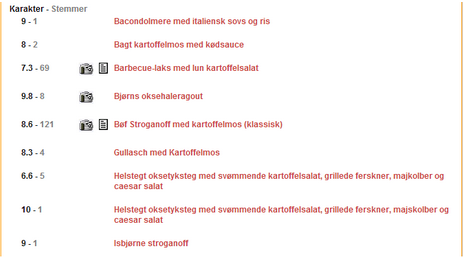
\includegraphics[scale=0.7]{billeder/forbilleder/dk-kogebogen2.png}
\capt{Liste af opskrifter, som indeholder ingredienserne Tomat, Paprika og Kartoffel.}
\label{fig:dk-kogebogen2}
\end{figure}

Brugeren vælger derefter en af opskrifterne han/hun finder mest interessant. Der er ikke overensstemmelse med, hvad \fx portionerne skal angives i. Inde på hjemmesiden er det i nogle tilfælde muligt at op- eller nedskalere portionsstørrelsen, mens der i andre tilfælde skaleres på antal personer. Derudover er der også nogle opskrifter, hvor det slet ikke er muligt at skalere. Her er brugeren i stedet for tvunget til selv at finde ud af, hvor stor en portion opskriften ca. passer til. Denne mangel på konsistens er endnu en af problematikkerne ved, at det er brugerne selv, som indsender opskrifterne. En endelig vurdering af DK-Kogebogen, vil kunne findes i \secref{subsec:eksisterende.sammendrag}.

\subsection{Opskrifter.dk}
\label{subsec:opskrifterdk}

Opskrifter.dk er endnu en webapplikation, der tilbyder en ``Tøm køleskabet''-funktion, som kan bruges til at finde opskrifter i deres samling af opskrifter. Ligesom i For Resten kan ingredienser kun vælges fra kategorier, dog er der i dette system hele 624 ingredienser, fordelt over 27 kategorier. Modsat For Resten kan man her vælge mere end én ingrediens. Dette gøres ved først at vælge en kategori og derefter finde og vælge en ingrediens og klikke på knappen ``Tilføj >''. Man kan ligeledes fjerne allerede valgte ingredienser ved at markere dem og klikke på knappen ``< Fjern'', eller fjerne alle valgte ingredienser ved at klikke på knappen ``< Fjern alle''. Når man har valgt de ingredienser, man ønsker at inkludere, kan man foretage sin søgning ved at klike på knappen ``Søg''. 

\begin{figure}[H]
\centering
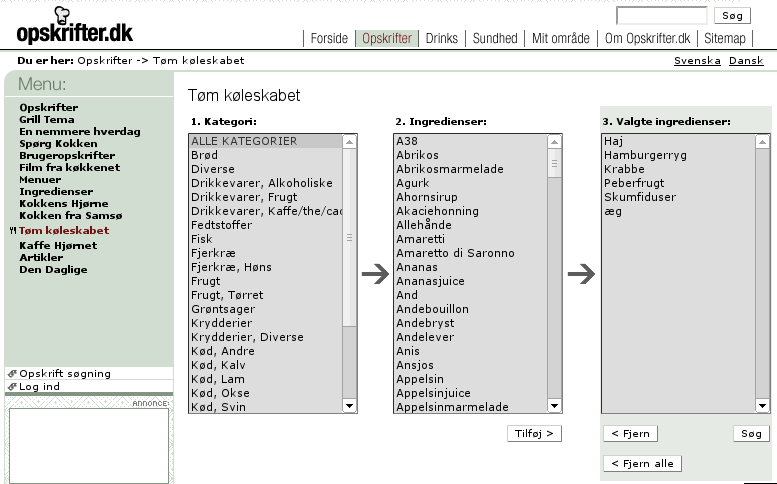
\includegraphics[scale=0.6]{billeder/forbilleder/opskrifterdk.png}
\capt{Brugergrænsefladen for Opskrifter.dk’s ``Tøm køleskabet''-funktion.}
\label{fig:opskrifterdk1}
\end{figure}

Søgningen foretages blandt de ca. 2700 opskrifter, som er tilgængelige på Opskrifter.dk. Resultaterne vælges ud fra, om de inkluderer minimum én af de valgte ingredienser. Under hver opskriftnavn vises antallet af valgte ingredienser, som opskriften inkluderer, men det er umiddelbart ikke muligt at sortere resultaterne efter dette tal. Klikker man på et resultat, åbnes den valgte opskrift til højre for resultaterne, og altså ikke på en ny side eller i et nyt vindue/faneblad. Opskrifterne viser informationer såsom tilberedningstid samt alle ingredienserne og deres mængder. Det er på alle opskrifter muligt at skalere opskriften til et bestemt antal personer. Figur \ref{fig:opskrifterdk2} viser et eksempel af et søgningsresultat. 

Kvaliteten af opskrifterne er forholdsvis høj og ca. 40 \% af alle opskrifter er med billede. Dette skyldes sandsynligvis, at det ikke er muligt for almindelige brugere direkte at indsende opskrifter. Almindelige brugere kan derimod indsende opskriftforslag, som først skal gennemlæses og tilføjes af en administrator.

\begin{figure}
\centering
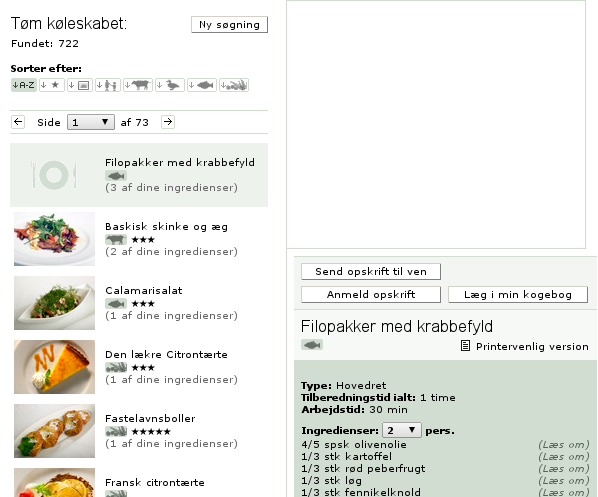
\includegraphics[scale=0.7]{billeder/forbilleder/opskrifterdk2.png}
\capt{Resultatsiden vist ved søgning med Opskrifter.dk’s ``Tøm køleskabet''-funktion. Her er markeret en opskrift, der ikke indeholder et billede af retten.}
\label{fig:opskrifterdk2}
\end{figure}

Opskrifter.dk har også et brugersystem, der tillader brugere at registrere sig og logge ind. Dette giver mulighed for, at man bl.a. kan gemme de opskrifter, man har fundet (ved at klikke på ``Læg i min kogebog''). Derudover husker ``Tøm køleskabet''-funktionen de ingredienser, man har indtastet, til næste gang man besøger siden.
Under ``Tøm køleskabet''-funktionen er det også muligt for brugeren at skrive kommentarer til funktionen. Disse kommentarer har givet et indblik i, hvad Opskrifter.dk’s brugere synes om funktionaliteten. Nogle kommentarer går på manglende ingredienser, mens en stor del kommentarer går på, at funktionen finder opskrifter, som man ikke kan lave uden at skulle købe en masse ind. \Fx skriver brugeren Jytte Hasselriis:

%kilde: http://opskrifter.dk/Toem-koeleskabet.149.0.html
\begin{quote}
``Hvordan skulle jeg kunne lave fasan i flødesovs, når jeg ikke har en fasan i køleskabet????'' \cite{opskrift-fasan}
\end{quote}

Dette synes at udtrykke en vis utilfredshed med den måde, hvorpå Opskrifter.dk’s ``Tøm køleskabet''-funktion vælger resultater på.
\subsection{Sammendrag}
\label{subsec:eksisterende.sammendrag}

De tre systemer; For Resten, DK-Kogebogen og Opskrifter.dk er i foregående afsnit blevet undersøgt og analyseret. Der er blevet lagt vægt på fire hovedpunkter: antallet af opskrifter i systemet, Kvaliteten af opskrifterne, systemets fleksibilitet og opskriftssøgningsfunktionen (også kaldet ``Tøm køleskabet''-funktionen). De fire hovedpunkter er specificeret i detaljer i \secref{sec:eksisterendesystemer}. For at skabe et samlet overblik, har vi valgt at samle de vigtigste og mest karakteristiske dele fra hver af systemerne i \tableref{table:sammentabel}.

\ourtable{sammentabel}{3}{Oversigt over opfyldelse af kriterier af de eksisterende systemer.}
                                            {System}
       { Funktioner                }{ For Resten   & DK-kogebogen   & Opskrifter.dk }{
\ourrow{ Kvalitet af opskrifter    }{ ringe        & svingende      & god           }
\ourrow{ Antal opskrifter          }{ 550          & 36.500         & 2.700         }
\ourrow{ Fleksibilitet             }{ meget ringe  & middel         & god           }
\ourrow{ Opskriftssøgningsfunktion }{ meget ringe  & middel         & middel        }
}

\begin{description}
\item[Kvalitet af opskrifter] \hfill \\
Kvaliteten af opskrifterne på DK-Kogebogen er meget varierende. Brugeren risikerer at støde på opskrifter, der slet ikke er brugelige. 

Kvaliteten af opskrifterne på For Resten kunne være meget bedre. Opskrifterne er udelukkende lavet eller tilføjet af folkene bag app’en, og derfor er opskrifternes opbygning og design konsistent, hvilket naturligvis havde været en god egenskab, hvis det ikke var for det faktum, at opbygningen er uoverskuelig, og at der ingen billeder eksisterer af opskriften. Der er ingen ingrediensliste på opskriften og beskrivelsen af fremgangsmåden er kortfattet. 

Kvaliteten af opskrifterne på Opskrifter.dk er høj. Dette skyldes, at opskrifterne bliver gennemgået af en administrator, inden de bliver tilgængelige på Opskrifter.dk’s side, hvilket er modsat af DK-Kogebogen, hvor opskrifterne bliver tilgængelige med det samme. Desuden er Opskrifter.dk’s opskriftsopbygning konsekvent i alle opskrifter, hvilket også er i modsætning til DK-Kogebogens opskrifter. Der mangler dog billeder på nogle opskrifter.

\item[Antal opskrifter] \hfill \\
Som det ses i \tableref{table:sammentabel}, har DK-Kogebogen det langt største antal opskrifter, mens Opskrifter.dk har ca. fem gange flere opskrifter end For Resten. Dermed har DK-Kogebogens ``Tøm køleskabet''-funktion også langt bedre chance for at give brugeren et resultat, når der søges på opskrifter med specifikke ingredienser.

\item[Fleksibilitet] \hfill \\
Der er stor forskel på fleksibiliteten fra system til system. I For Restens app, er det slet ikke muligt at skalere portionsstørrelse. På DK-Kogebogens side er det kun muligt med nogle opskrifter, mens det på Opskrifter.dk er muligt at skalere portionsstørrelse i alle opskrifter. Denne relativ simpel funktion ses som meget brugbar, da brugeren undgår selv at skulle gange ingrediensmængder op.

Kun Opskrifter.dk tilbyder brugeren muligheden for at sortere i resultaterne af en opskriftssøgning. Her kan der sorteres efter alfabetisk orden, opskrifter med billeder, opskrifter med kød samt flere. Som en bruger på Opskrifter.dk dog pointere, mangler den sorteringsmulighed, som sortere efter de opskrifter som indeholder flest af de ingredienser som brugeren har indtastet. Denne sorteringsmulighed anses for os, som værende den mest relevante, da man som bruger er interesseret i at få anvendt så mange af ens madrester som muligt.

\item[Opskriftssøgningsfunktion] \hfill \\
De tre systemer er vidt forskellige i deres måde at håndtere søgning på. Der er mellem DK-kogebogen og Opskrifter.dk en markant forskel på, hvordan resultater findes. I DK-Kogebogen findes kun opskrifter, som inkluderer alle de indtastede ingredienser, mens Opskrifter.dk finder alle opskrifter, som indeholder bare én af de valgte ingredienser. Dvs., at man med DK-Kogebogen får færre resultater jo flere ingredienser man skriver, mens det med Opskrifter.dk er direkte modsat, idet antallet af resultater stiger voldsomt med antallet af ingredienser, man skriver. Opskrifter.dk’s måde at gøre det på, kombineret med deres manglende sortering, giver en uoverskuelig mængde af resultater, hvor en stor del af disse måske kun indeholder en af de valgte ingredienser.
\end{description}

%Ud fra vores observationer af løsningernes fordele og ulemper, kan vi uddrage hvilke egenskaber vi ønsker at benytte i vores eget projekt. \Fx viser den generelle utilfredshed med Forbrugerstyrelsens mobilapp For Resten, at det er vigtigt med mange opskrifter og muligheden for at vælge mere end én rest. Observationerne af For Resten og Opskrifter.dk viser også, at brugergrænseflade er et vigtigt element. I disse to løsninger skal man vælge ingredienser ved at lede rundt i kategorier. Dette føles meget ineffektivt i forhold til at skrive navnet på ingrediensen på et tastatur.

%Af dette kan man aflede, at en kombination af de to må være den optimale løsning. Har man valgt få ingredienser, er man sandsynligvis interesseret i at få vist resultater som indeholder alle de ingredienser man har valgt. Har man derimod valgt mange ingredienser, er man interesseret i at få vist resultater som indeholder flest muligt af de ingredienser man har valgt.

%Som det ses i \tableref{table:sammentabel}, har DK-Kogebogen det langt største antal opskrifter, mens Opskrifter.dk har ca. fem gange flere opskrifter end For Resten. Dermed har DK-Kogebogens ``Tøm køleskabet''-funktion også langt bedre chance for at give brugeren et resultat, når han/hun søger på opskrifter med specifikke ingredienser. Til gengæld er kvaliteten af opskrifterne på DK-Kogebogen meget varierende, og derfor kan brugeren risikere at støde på opskrifter, som er dårlige eller ubrugelige. Kvaliteten af opskrifterne på For Resten er sammenlagt dårlig. Opskrifterne er udelukkende lavet eller tilføjet af folkene bag app’en, og derfor er opskrifternes opbygning og design konsistent, hvilket naturligvis havde været en god egenskab, hvis det ikke var for det faktum, at opbygningen er uoverskuelig. Der er ingen ingrediensliste på opskriften og beskrivelsen af fremgangsmåden er kortfattet. Kvaliteten af opskrifterne på Opskrifter.dk er høj. Dette skyldes, at opskrifterne bliver gennemgået af en administrator, inden de bliver tilgængelige på Opskrifter.dk’s side, hvilket er modsat af DK-Kogebogen, hvor opskrifterne bliver tilgængelige med det samme. Desuden er Opskrifter.dk’s opskriftopbygning konsekvent i alle opskrifter, hvilket også er i modsætning til DK-Kogebogens opskrifter.

%Der er stor forskel på fleksibiliteten fra system til system. I For Restens app, er det slet ikke muligt at skalere portionsstørrelse. På DK-Kogebogens side er det kun muligt med nogle opskrifter, mens det på Opskrifter.dk er muligt at skalere portionsstørrelse alle opskrifter. Det er en funktion, som er meget brugbar, da man som bruger ikke ønsker at bruge en masse tid på selv at beregne en passende portionsstørrelse. Af sorteringsmuligheder af opskriftresultaterne, er det kun Opskrifter.dk som tilbyder denne mulighed. Her kan der sorteres efter alfabetisk orden, opskrifter med billeder, opskrifter med kød samt flere. Som en bruger på Opskrifter.dk dog pointere, mangler den sorteringsmulighed, som sortere efter de opskrifter som indeholder flest af de ingredienser som brugeren har indtastet. Denne sorteringsmulighed anses for os, som værende den mest relevante, da man som bruger er interesseret i at få anvendt så mange af ens madrester som muligt. 

%De tre løsninger er vidt forskellige i deres måde at håndtere søgning på. Ud fra vores afprøvninger og observationer af løsningernes fordele og ulemper, kan vi uddrage hvilke egenskaber vi ønsker at benytte i vores eget projekt. \Fx viser den generelle utilfredshed med Forbrugerstyrelsens mobilapp For Resten, at det er vigtigt med mange opskrifter og muligheden for at vælge mere end en rest. Observationerne af For Resten og Opskrifter.dk viser også at brugergrænseflade er et vigtigt element. I disse to løsninger skal man vælge ingredienser ved at lede rundt i kategorier og i For Resten endda bevæge fingeren rundt i en cirkel for at rotere hjulene for kategorier og rester. Dette føles meget ineffektivt i forhold til at skrive navnet på ingrediensen på et tastatur. Derudover er der mellem DK-kogebogen og Opskrifter.dk en markant forskel på hvordan resultater findes. I DK-kogebogen findes kun opskrifter som inkluderer alle de indtastede ingredienser, mens Opskrifter.dk finder alle opskrifter som indeholder bare én af de valgte ingredienser. Dvs. at man med DK-kogebogen får færre resultater jo flere ingredienser man skriver, mens det med Opskrifter.dk er direkte modsat, idet antallet af resultater stiger voldsomt med antallet af ingredienser man skriver. Opskrifter.dk’s måde at gøre det på, kombineret med deres manglende sortering, giver et stor uoverskuelig mængde af resultater, hvor en stor del af disse måske kun indeholder en af de valgte ingredienser. Af dette kan man aflede at en kombination af de to må være den optimale løsning. Har man valgt få ingredienser, er man sandsynligvis interesseret i at få vist resultater som indeholder alle de ingredienser man har valgt. Har man derimod valgt mange ingredienser, er man interesseret i at få vist resultater som indeholder flest muligt af de ingredienser man har valgt.


\section{Systemdefinition}

%Systemdefinitionen nedenunder er en naturlig og kortfattet beskrivelse af den løsning, vi ønsker at fremstille. Den er baseret på gruppens egne ønsker om projektretning og interviews med gruppens to informanter. BATOFF-modellen er blevet brugt til at formulere systemdefinitionen. BATOFF indeholdholder følgende punkter: \emph{\textbf{b}etingelser}, \emph{\textbf{a}nvendelsesområde}, \emph{\textbf{t}eknologier}, \emph{\textbf{f}unktioner}, \emph{\textbf{f}ilosofi}. Gruppen benytter BATOFF-modellen fordi det fastsætter nogle rammer i forhold til opsætningen og indholdet af systemdefinitionen samt opretter en form for standard, der gør det muligt at sammenligne flere forskellige systemdefinitioner på en logisk måde.

%Efter møde 1 (se bilag) med vores informanter, har gruppen fået forståelse for at madspild er et reelt problem for dem. Det er blevet forklaret hvad der ofte er grunden til madspildet, og på baggrund af møde 1 er to systemdefinitioner blevet konstrueret. Blandt de to systemdefinitioner valgte informanterne systemdefinition 1. Systemdefinition 2 kan ses i den akademiske rapport.

%Systemdefinition er defineret som følgende:

%\begin{quote}
%Systemet skal fungere som et online opskriftsregister, der giver brugeren idéer til opskrifter han rent faktisk kan lave ud fra de madvarer han har. Systemet fokuserer på at mindske madspild, da forbrugere smider mad ud på grund af et manglende formål med anvendelsen af resterne. Brugerne af programmet er en del af en husholdning og vil have meget varierende erfaringer inden for brug af internettet. Udviklerne af systemet er ulønnede studerende. Deadline for det færdige system kan ikke ændres. Systemet skal køre på en server, der kan tilgås via en webapplikation fra en internetbrowser på enhver type computer. På baggrund af en mængde fødevarer som input, findes forskellige opskrifter, der bedst muligt matcher disse. Opskrifterne skal kunne sorteres på flere måder, og ingredienser skal kunne huskes til næste gang, hvis ønsket.
%\end{quote}

%Gruppen mødtes anden gang med informanterne efter at have fremstillet de to systemdefinitioner for at få feedback på projektets retning og få valgt et attraktivt systemdefinition. Formålet med mødet er at fortælle informanterne om gruppens idé om en opskriftssøgemaskine, der kun finder opskrifter man kan lave ud fra de råvarer, man har til rådighed. Gruppen vil høre om informanterne ville kunne bruge et sådan system. Gruppen holder sig på nuværende tidspunkt meget åbent, da gruppen vil gerne gøre det muligt for informanterne at komme med nye idéer, også selvom de er markant anderledes fra gruppens initierende problemstilling og systemdefinitioner. Derfor foregår mødet som et semistruktureret interview. Det er vigtigt for gruppen at få informanternes idéer til hvilke funktioner et sådan system skal have og hvilken krav, de stiller.

%Møde 2 gjorde det klart, at informanterne ser systemdefinition 1 som et meget brugbart system. Vi er blevet præsenteret for en masse funktioner, som hver informant har ønsket til et sådan system.

%Dokumentation og referater fra møde 1 og 2 samt alle efterfølgende møder med informanterne kan findes i \apref{ap:informant}.
